\chapter{The LHC and CMS Machine} % (fold)
\label{cha:the_lhc_and_cms_machine}

In this chapter, the working and the design parameters of \acrfull{lhc} and its one of main purpose detector, Compact Muon Solenoid (CMS), are briefly described.


%%%%%%%%%%%%%%%%%%%%%%%%%%%%%%%%%%%%%%%%%%%%%%%%%%%%%%%%%%%%%%%%%%
\section{The Large Hadron Collider} % (fold)
\label{sec:the_large_hadron_collider}

The famous quote ``history repeats itself" applies well to the \acrfull{hep} experiments. The starting point of experimental particle physics is the Rutherford $\alpha$-particle scattering, which is suggested by Ernest Rutherford and carried out by the two assistant  Hans Geiger and Ernest Marsden in early 20th century~\cite{Hauptman2010}. In this experiment Rutherford suggested to aim the beam of $\alpha$-particles to the thin gold foil and using the experimental findings they suggested the well known structure of today's atom, in which the most of mass centered at core of atom which is known as nucleus and the electrons  rotates around the nucleus. Even now we are doing the same thing just the method changed from ``natural accelerator"\footnote{radioactivity and cosmic rays} to the ``man-made" accelerator that can accelerate particles with the velocity close to the speed of light. The design and working of the accelerator has changed a lot over a period of time in going from MeV to GeV and in the TeV range. Now, these machines are not only used in \acrshort{hep} experiments, but also extends their arenas to treating human beings from cancer therapy, radioisotope production, 3-D x-ray\todo[fancyline]{Add citations to the applications}, also to the industry for uses like material processing, sterilization, security scan, water treatment, and many more. 

The \acrshort{lhc} is  a hadron collider which can accelerate two proton beams, moving in opposite direction, to a maximum of 14 TeV energy in a 26.6 km long tunnel which is about 100 m underground. The \acrshort{lhc} is the latest and most-powerful accelerator everbuilt. It is a proton-proton collider built to improve our understanding of fundamental physics. It started on 21$^{st}$ October 2008 and is positioned in the samee tunnel that earlier had Large Electron Positron Collider (LEP). The LEP collaboration decided to switch to hadron collider because of following advantages:
\begin{itemize}
    \item Hadron collider can reach a higher Center Of Mass (COM) energy, because of much lower synchrotron radiation \footnote{The radiation emitted by a charged particle during acceleration in a circular path is known as synchrotron radiation. As the particles loses energy in emission of this radiation an additional energy must be provided to keep the beam at constant energy.} emitted by hadrons as compared to electrons. Synchrotron radiation loss is directly proportional to $(Energy/mass)^4$. \todo[fancyline]{Add exact number for electrons and protons synchrotron loss.}
    \item As hadrons are composite particles, they allow us to scan over wide range of energies.
\end{itemize}


For any particle accelerator, there are mainly three components. In case of LHC, they are:
\begin{itemize}
  \item Beam pipes
  \item Accelerating structure
  \item Magnet system
\end{itemize}

%%%%%%%%%%%%%%%%%%%%%%%%%%%%%%%%%%%%%%%%%%%%%%%%%%%%%%%%%%%%%%%%%%
%%%%%%%%%%%%%%%%%%%%%%%%%%%%%%%%%%%%%%%%%%%%%%%%%%%%%%%%%%%%%%%%%%
\subsection{Beam Pipes} % (fold)
\label{sub:beam_pipes}

At LHC, there are two beam pipes each with diameter $\approx$6.3 cm in which proton beams travel in opposite directions. To avoid beam instability and loss of beam particles due to collision with gas molecules; the beam pipes are kept at ultra-high vacuum\footnote{At LHC, three different vacuum systems are used. First one is used for beam pipe; second one for insulating the cryogenically cooled magnets and third one is used for insulating the helium distribution. In the latter two it just acts as a thermal insulator as the cryogenic parts are kept at 1.9 K ($\ang{-271.3}C$)} $1.013 \times 10^{-13}$ bar pressure.
% subsection beam_pipes (end)

%%%%%%%%%%%%%%%%%%%%%%%%%%%%%%%%%%%%%%%%%%%%%%%%%%%%%%%%%%%%%%%%%%
%%%%%%%%%%%%%%%%%%%%%%%%%%%%%%%%%%%%%%%%%%%%%%%%%%%%%%%%%%%%%%%%%%
\subsection{Accelerating Structure} % (fold)
\label{sub:accelerating_structure}

Another main part of any particle accelerator is its accelerating structure. A accelerator in the TeV range can not start from rest and go to the TeV range in one go; it should go into several stages depending on the energy. At LHC, the journey of proton starts with grabbing the proton from Hydrogen gas and subsequently going into 5 different stages. The stages can be decreased but could not be decreased to just one. Here, at LHC there are five different stages before reaching to LHC and in between it serves several other experiments at each stage, which are shown pictorially in Figure~\ref{fig:OtherExpAtAccStructure}. The stages for proton acceleration are:
\begin{itemize}
    \item Grab proton source: The source of proton is Duoplasmatron\footnote{It strips electron from hydrogen gas and creates a plasma of protons, electrons and molecular ions. This plasma expands towards the extraction electrodes and a proton beam is formed}\cite{LHC-tdr-vol3}. This feeds protons to LINAC2.
    \item LINAC2 (Linear accelerator-2): It is the starting point of proton's journey in the LHC accelerator complex. Here, protons reaches to an energy of 50 $MeV$ using the radio-frequency (RF) cavities\footnote{A RF cavity is an metallic cavity that accelerates the charged particles using the electromagnetic field.} where they also gains 5\% in mass. LINAC2 further feeds to the Proton Synchrotron Booster (PSB).
    \item PSB: It takes 50 $MeV$ proton beams from LINAC2 and accelerate them to 1.4 $GeV$ for injection into Proton Synchrotron (PS).
    \item PS: It is one of key component in the LHC accelerator complex. It increases the energy of protons up-to 25 $GeV$ and feeds to super proton synchrotron.
    \item Super Proton Synchrotron (SPS): It has a circumference of 7 $km$ where protons are accelerated to an energy of 450 $GeV$. Then via two transmission line protons are then injected into LHC ring.
    \item LHC: It grabs two proton beams from SPS which are injected into opposite directions in parallel pipes. In LHC, proton beams can be accelerated up-to 7 $TeV$.
\end{itemize}
The CERN accelerator complex is shown in Figure~\ref{fig:CERN-accelerator-complex}.  

% subsection accelerating_structure (end)
\begin{figure}[!htbp]
	\centering
	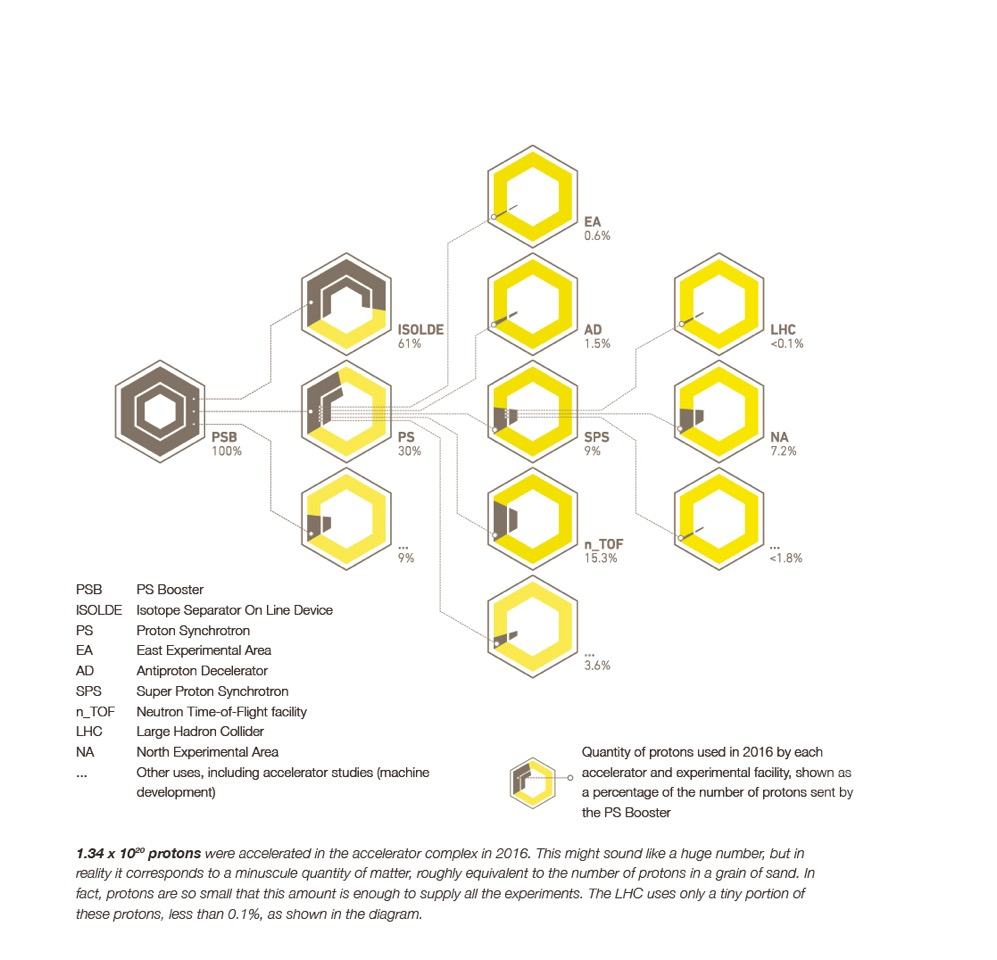
\includegraphics[width=1.0\textwidth]{figures/LHC/distribution_of_protons_en.jpg}
	\caption{Other experiments at the LHC accelerating chain \cite{OtherExpAtLHCAcceleratingChain}}
	\label{fig:OtherExpAtAccStructure}
\end{figure}
\begin{figure}[!htbp]
	\centering
	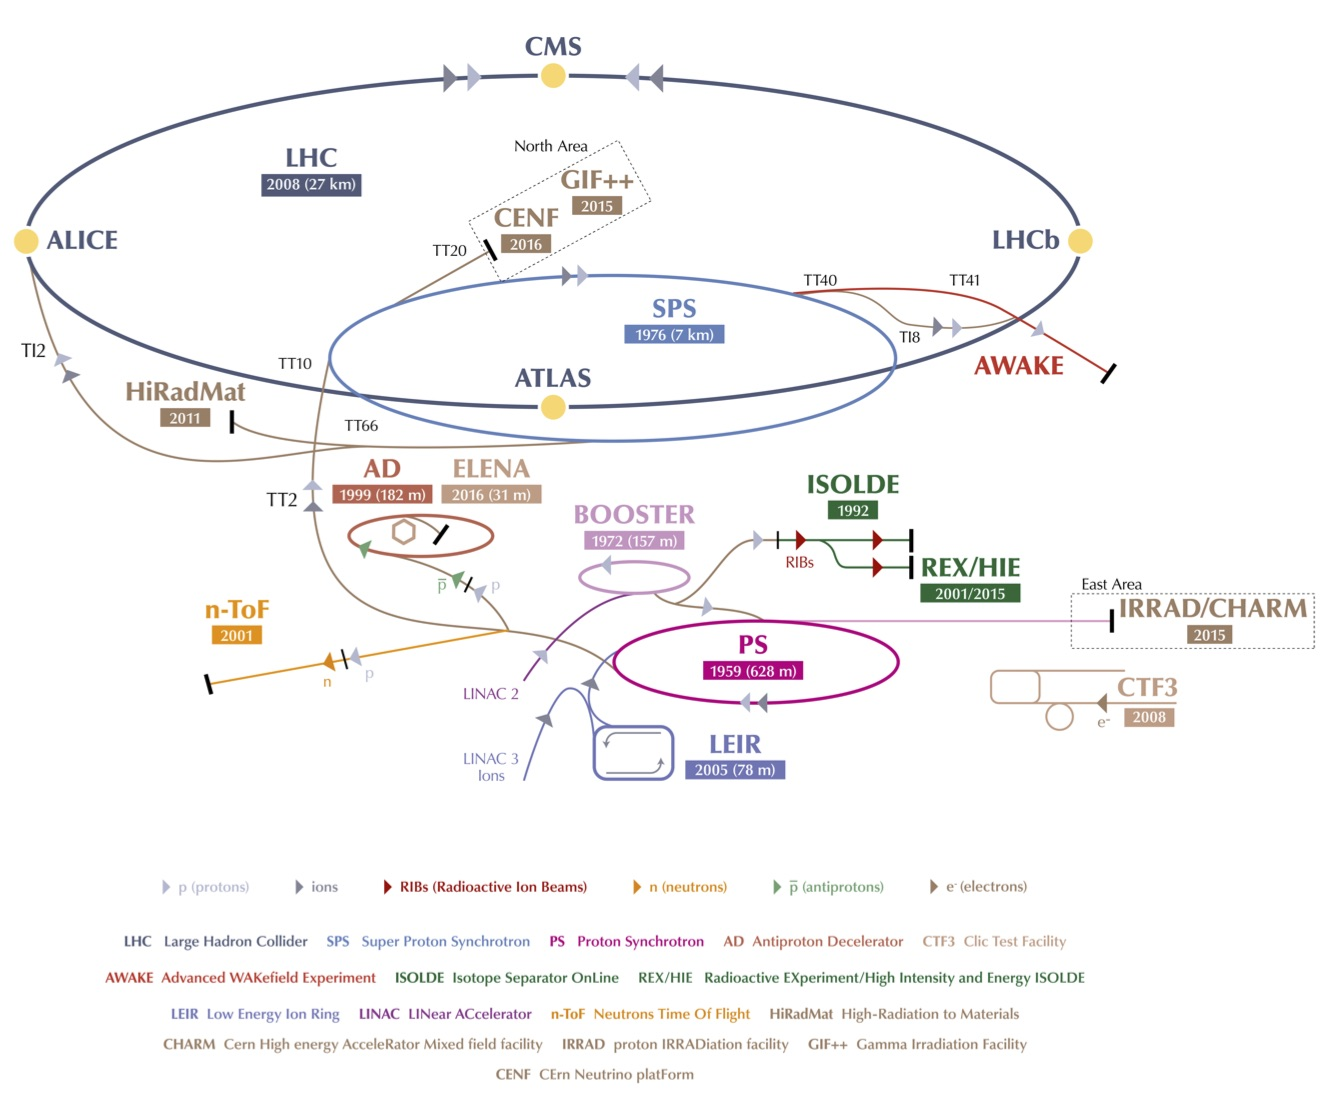
\includegraphics[width=1.35\textwidth]{figures/LHC/CERN_Accelerator_Complex-v2016.jpg}
	\caption{LHC accelerator chain along with all its other experiments which uses proton beam from other part of accelerator either from PSB, PS or SPS\cite{Fig-CERN-accelerator-complex}}
	\label{fig:CERN-accelerator-complex}
\end{figure}
%%%%%%%%%%%%%%%%%%%%%%%%%%%%%%%%%%%%%%%%%%%%%%%%%%%%%%%%%%%%%%%%%%
%%%%%%%%%%%%%%%%%%%%%%%%%%%%%%%%%%%%%%%%%%%%%%%%%%%%%%%%%%%%%%%%%%
\subsection{Magnet System}
As the LHC is a circular collider; magnet system is one of the core parts and gives particles a circular trajectory in the LHC beam pipes. To be economical LHC has been made in eight arcs and eight straight sections instead of a perfect circle. Apart from bending the beam, it is also necessary to focus the beam as the same charge protons try to diverge. To focus the beam a pair of quadrapole magnets is used. One focuses the beam width while other focuses the beam height. Quadrapole magnet geometry is shown in Figure~\ref{fig:QuadrupoleMagnet}. A total of 858 quadrupole magnets are installed in LHC to keep the beam focused. Sextupole magnets are also used for proper focusing as every proton in the beam is not exactly with the same energy and on thee same path. Several other magnetic multi-poles are used to keep the beam focused  in case the beam suffers from gravitational interactions over protons, electromagnetic interactions among bunches, electron clouds from pipe wall, and so on. Different types of magnets used in LHC are listed here \cite{WebLink:LHC_magnets}. Besides, there are eight sets of ``inner triplets" used at the four interaction points (IPs) to focus the beams while colliding to increase the luminosity. Here the size of bunch goes from 0.2 mm to 17 $\mu m$ at the interaction point of ATLAS or CMS. At the interaction point of ALICE or LHCb it is 71 $\mu m$. Summary of important parameters of LHC is given in Table~\ref{table:LHC-parameters}.
\begin{figure}[!htbp]
	\centering
	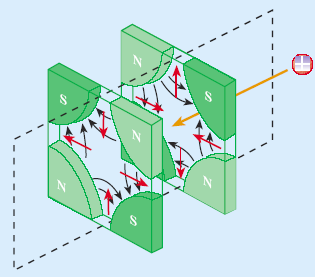
\includegraphics[width=0.65\textwidth]{figures/LHC/quadrupole_magnet_pair.png}
	\caption{Pair of quadrupole magnets.}
	\label{fig:QuadrupoleMagnet}
\end{figure}
% \begin{figure}[!htbp]
% 	\centering
% 	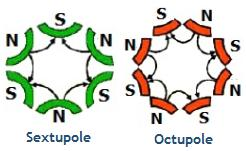
\includegraphics[width=0.95\textwidth]{figures/LHC/sextupole-octupole.jpg}
% 	\caption{Sextupole and octupole}
% 	\label{fig:sextupole-octupole}
% \end{figure}



\begin{table}
\centering
\begin{tabular}[!htbp]{l c}
\hline
{\bf Parameters} & {\bf Value} \\
\hline
Circumference of LHC ring   &   26658.883 m \\
\hline
Maximum dipole magnetic field   & 8.33 T \\
Dipole operating temperature    & 1.9 K \\
\hline
Maximum stored energy per beam (nominal) &   362 MJ \\
Maximum stored energy per beam  (2012) &   143 MJ \\
Maximum stored energy per beam  (2016) &   266 MJ \\
\hline
Beam energy at Injection    & 450 GeV \\
Beam energy at collision (nominal) &    7 TeV \\
Beam energy at collision (2012)     &   4 TeV \\
Beam energy at collision (2016)     &   6.5 TeV \\
\hline
Maximum instantaneous luminosity (nominal)  &   $10^{34}$ cm$^-2$ s$^{-1}$ \\
Maximum instantaneous luminosity (2012)     &   $7.7 \times 10^{33}$ cm$^-2$ s$^{-1}$ \\
Maximum instantaneous luminosity (2016)     &   $1.4 \times 10^{34}$ cm$^-2$ s$^{-1}$ \\
\hline
Number of bunches per proton beam (nominal) &   2808 \\
Number of bunches per proton beam (2012)    &   1380 \\
Number of bunches per proton beam (2016)    &   2076 \\
Maximum number of protons per bunch         &   $1.6 \times 10^{11}$ \\
\hline
Protons/bunch (average at start of collision) (nominal)   &   $1.15 \times 10^{11}$ \\
Protons/bunch (average at start of collision) (2012)  &   $1.5 \times 10^{11}$ \\
Protons/bunch (average at start of collision) (2016)  &   $1.1 \times 10^{11}$ \\
\hline
Bunch collision frequency (nominal)         &   40 MHz  \\
Bunch collision frequency (2012)            &   20 MHz  \\
Bunch collision frequency (2016)            &   40 MHz  \\
\hline
Bunch length (at injection)   &   1.7 ns \\
Bunch length (at collision)   &   1.05 ns \\
Energy spread (at injection)   &   1.9$\times 10^{-3}$ \\
Energy spread (at collision)   &   0.45$\times 10^{-3}$  \\
\hline
Half crossing angle  (nominal)   & 143 $\mu rad$ \\
Half crossing angle  (2012)   & 146 $\mu rad$ \\
Half crossing angle  (2016)   & 185 $\mu rad$ \\
\hline
$\beta *$  (nominal) &   0.55 m\\
$\beta *$   (2012)&   0.6 m\\
$\beta *$   (2016)&   0.4 m\\
\hline
RMS beam size at IP1 \& IP5 &   17 $\mu m$ \\
RMS beam size at IP2 \& IP8 &   71 $\mu m$ \\
\hline
$\epsilon_n$(transverse emittance, rms, normalized) (at injection) &   3.5 $\mu$m\\
$\epsilon_n$(transverse emittance, rms, normalized) (at collision point) &   3.75 $\mu$m\\
\hline
total longitudinal emittance (at injection) & 1.0 eVs \\
total longitudinal emittance (at collision) & 2.5 eVs \\
\hline
Average mean pile-up (nominal) &   25 \\
Average mean pile-up (2012) &    20 \\
Average mean pile-up (2016) &    40 \\
\hline
Energy loss per turn at 14 TeV              &   7 keV   \\
Energy loss per turn for electrons at 104.6 GeV          &  40,000 keV     \\
% synchtron radiation for electrons: Reference: Particle Physics Experiments at high energy colliders by John Hauptman
\end{tabular}
\caption{LHC technical parameters for proton-proton collisions: nominal, 2012 and 2016 values.\cite{Bruce2016, Schoerner-Sadenius2015, LHC-parameters-2016, LHC-tdr-vol1}.}
\label{table:LHC-parameters}
\end{table}

%%%%%%%%%%%%%%%%%%%%%%%%%%%%%%%%%%%%%%%%%%%%%%%%%%%%%%%%%%%%%%%%%%
%%%%%%%%%%%%%%%%%%%%%%%%%%%%%%%%%%%%%%%%%%%%%%%%%%%%%%%%%%%%%%%%%%
\subsection{Few key requirements} % (fold)
\label{sub:few_key_requirements}

The HEP collider is mainly characterized by the two parameters: center of mass (COM) energy and the luminosity. The production rate of heavier particles like Higgs increases with COM energy. The luminosity is proportional to the number of events per second so it should be maximized. Luminosity is defined as:
\begin{equation}
    L = \frac{k_bN_b^2f_{rev}\gamma}{4 \pi \epsilon_n \beta^*}
\end{equation}
where,\\
\hspace{2cm}$k_b$ is the number of bunches per ring,\\
\hspace{2cm}$N_b$ is the number of protons per bunch,\\
\hspace{2cm}$f_{rev}$ the revolution frequency,\\
\hspace{2cm}$\epsilon_n$ is the normalized RMS transverse beam emittance (same in both )\\
\hspace{2cm}$\beta^*$ is the beta-function at the interaction point\\

Based on the definition of luminosity, we can maximize it by following means:
\begin{itemize}
    \item By decreasing beam emittance, $\epsilon_n$.
    \item By improving the cryogenic system. As the factor $k_b.N_b$ is limited by thermal energy produced by synchrotron radiation.
    \item By decreasing beam-beam effect\todo[fancyline]{add reference of beam-beam effect}. As it scales with $N_b/ \epsilon_n$ which causes the spread in betatron tunes\todo[fancyline]{add reference of betatron tunes}.
    \item Also, the space charge \todo[fancyline]{add Reference of space-charge} scales with $N_b/ \epsilon_n$.
\end{itemize}
% subsection few_key_requirements (end)

% section the_large_hadron_collider (end)

%%%%%%%%%%%%%%%%%%%%%%%%%%%%%%%%%%%%%%%%%%%%%%%%%%%%%%%%%%%%%%%%%%
\section{Experiments at the LHC} % (fold)
\label{sec:experiments_at_the_lhc}

In LHC there are four IPs where two proton beams are made to collide. At every IP one detector is placed. They are ATLAS, CMS, ALICE, and LHCb as shown in Figure~\ref{fig:LHCgeometry}. Also, there are two more small detectors LHCf and TOTEM installed close to the IP of the two main detectors ATLAS and CMS respectively.
\begin{figure}[!htbp]
	\centering
	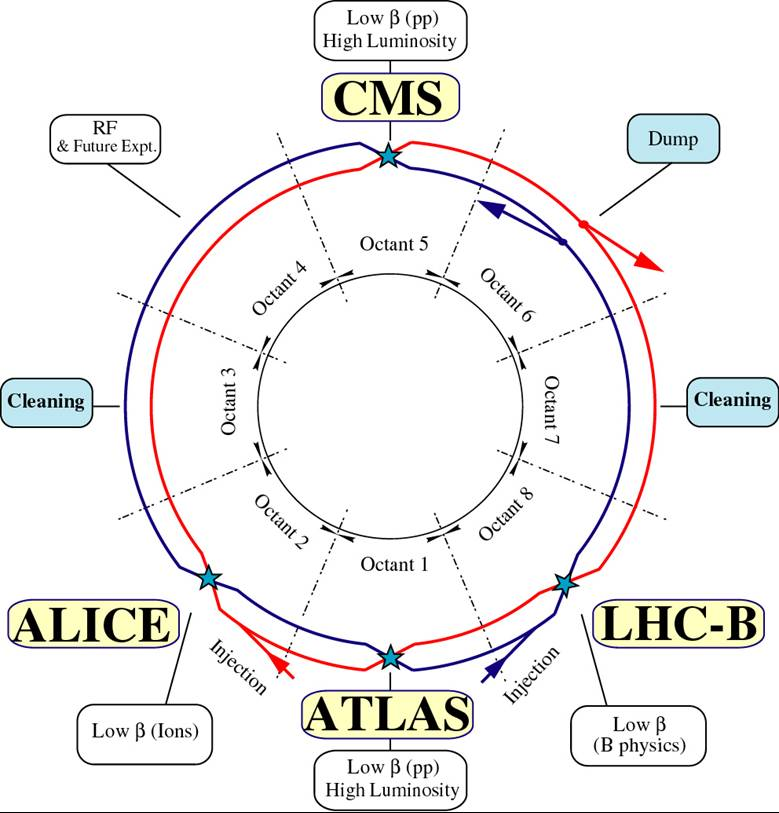
\includegraphics[width=0.95\textwidth]{figures/LHC/lhc-schematic.jpg}
	\caption{LHC geometry with arcs and straight sections.}
	\label{fig:LHCgeometry}
\end{figure}
\newline
{\bf ATLAS} (A Toroidal LHC Apparatus) and {\bf CMS} (Compact Muon Solenoid) are large general-purpose\footnote{Here, general purpose means this machines will be used for many different kind of physics searches.} detectors having similar design and similar goal. CMS detector will be described in detail in Section~\ref{sec:cms_experiment}. The main difference in the two is in their magnet systems. One additional choice that affects this is the momentum resolution for muons. The momentum resolution for muons, $\Delta p_T/p_T$, are proportional to  $B^{-1}L^{-2}$, where B is magnetic field and L is distance of momentum measurement from the IP of detector. So, To improve the momentum resolution there are two possible choices.

\begin{enumerate}
	\item Increase the magnetic field with compact design, or
	\item Work with low magnetic field with long lever arm, L
\end{enumerate}

There is also a third possibility to improve the momentum resolution by increasing the leaver arm as well as magnetic field, but it increases the cost of the detector by several factors. So, CMS chooses the first point, i.e., to increase the magnetic field with compact design\footnote{This is why there is word {\bf compact} in the name of CMS.} while ATLAS chooses the design with low magnetic field with long lever arm.

% ATLAS has an eight toroidal magnets combined with a smaller inner solenoid while CMS has a powerful solenoid magnet only.

{\bf ALICE} (A Large Ion Collider Experiment) is a heavy-ion detector. It is specially designed for the study of strongly interacting matter at high densities in quark-gluon plasma phase.

{\bf LHCb} (Large Hadron Collider beauty) is made asymmetrically with respect to the IP of the detector. It is made specially to study the slight differences between the matter-antimatter through the study of b-quarks.

{\bf LHCf} (Large Hadron Collider forward) and {\bf TOTEM} (TOTal cross-section, Elastic scattering and diffraction dissociation Measurement at the LHC) are located near ATLAS and CMS respectively, for the study of forward physics.
% section experiments_at_the_lhc (end)

% %%%%%%%%%%%%%%%%%%%%%%%%%%%%%%%%%%%%%%%%%%%%%%%%%%%%%%%%%%%%%%%%%%
\section{CMS Experiment} % (fold)
\label{sec:cms_experiment}
In a HEP detectors there are two different categories of conditons are imposed. They are:

\begin{itemize}
	\item restrictions imposed from the accelerator conditions.
	\item restrictions because of physics goal.
\end{itemize}

% While designing a HEP detector we need to take into account the environment created by the two proton-proton collision at LHC. So, the restriction imposes on detectors from LHC enviornment are

Restrictions imposed on detector from the LHC are:

\begin{itemize}
	\item \textbf{High luminosity delivered by LHC:} As the delivered luminosity is high this implies every-time the two proton bunches cross each other there will be more than one p-p interactions\footnote{More than one p-p interaction in one bunch crossing is known as pile-up. It is also given as the product of inelastic p-p cross-section ($\sigma_{inel}$), instantaneous luminosity ($L$) and the mean time interval between two collision, ($< t >$). \begin{equation}
		mean~pile-up = \sigma_{inel} \times L \times <t>
	\end{equation}}. This is one of greatest challenges. This implies more than 1000 particles passes through detector. This imposes condition that the detector should be highly granular this results with increase number of channels that should be synchronized with each other.
	\item \textbf{Event rate:} At LHC, the two proton bunches crosses each other at every 25 ns. So, the response time for all the sub-system of detector should be less than 25 ns.
	\item \textbf{Produced radiation:} At every 25ns the detectors are bombarded with more than 1000 particles so all the sub-detectors should be radiation hard including its electronics, cables, glue, screws, and so on.
\end{itemize}

Restrictions imposed on detector from physics goal are:

\begin{itemize}
	\item Good muon identification and momentum resolution ($\approx$ 1\% at 100 GeV).
	\item EEfficient triggering and tracking of b-jets and $\tau$'s.
	\item High resolution electromagnetic calorimeter to detect electrons and photons.
	\item Good missing transverse energy resolution and di-jet mass resolution requires a ``hermetic'' hadron calorimeter with full geometric coverage and fine lateral segmentation.
\end{itemize}

% When the two beam of proton collides then thousands of particles are produced and out of them only 9 particles are of interest from detector construction point of view. They are photons ($\gamma$), electrons ($e$), muons ($\mu$), pions ($\pi^{\pm}$), kaon ($K^{\pm},~K_L,~K_S$), protons ($p$), and neutrons ($n$). Out of rest there are three neutrinos which interacts only weakly that do not interact in light mass HEP detectors and others are short lived particles. So, 

Based on the above condition CMS detector was designed in cylindrical shape having each detector one on top of other with beam pipe at center. To have full geometric coverage it is designed with a barrel region and two endcap regions. Main part of the CMS detector is its superconducting magnet system with a high magnetic field of 4 Tesla to accurately measure the high momentum particles and its muon system. Muon system kept outside the magnet but sandwiched in its return yoke. While the tracking system and calorimeters are placed inside the magnet. CMS detector design is shown in Figure~\ref{fig:CMS-detector}.
\begin{figure}[!htbp]
	\centering
	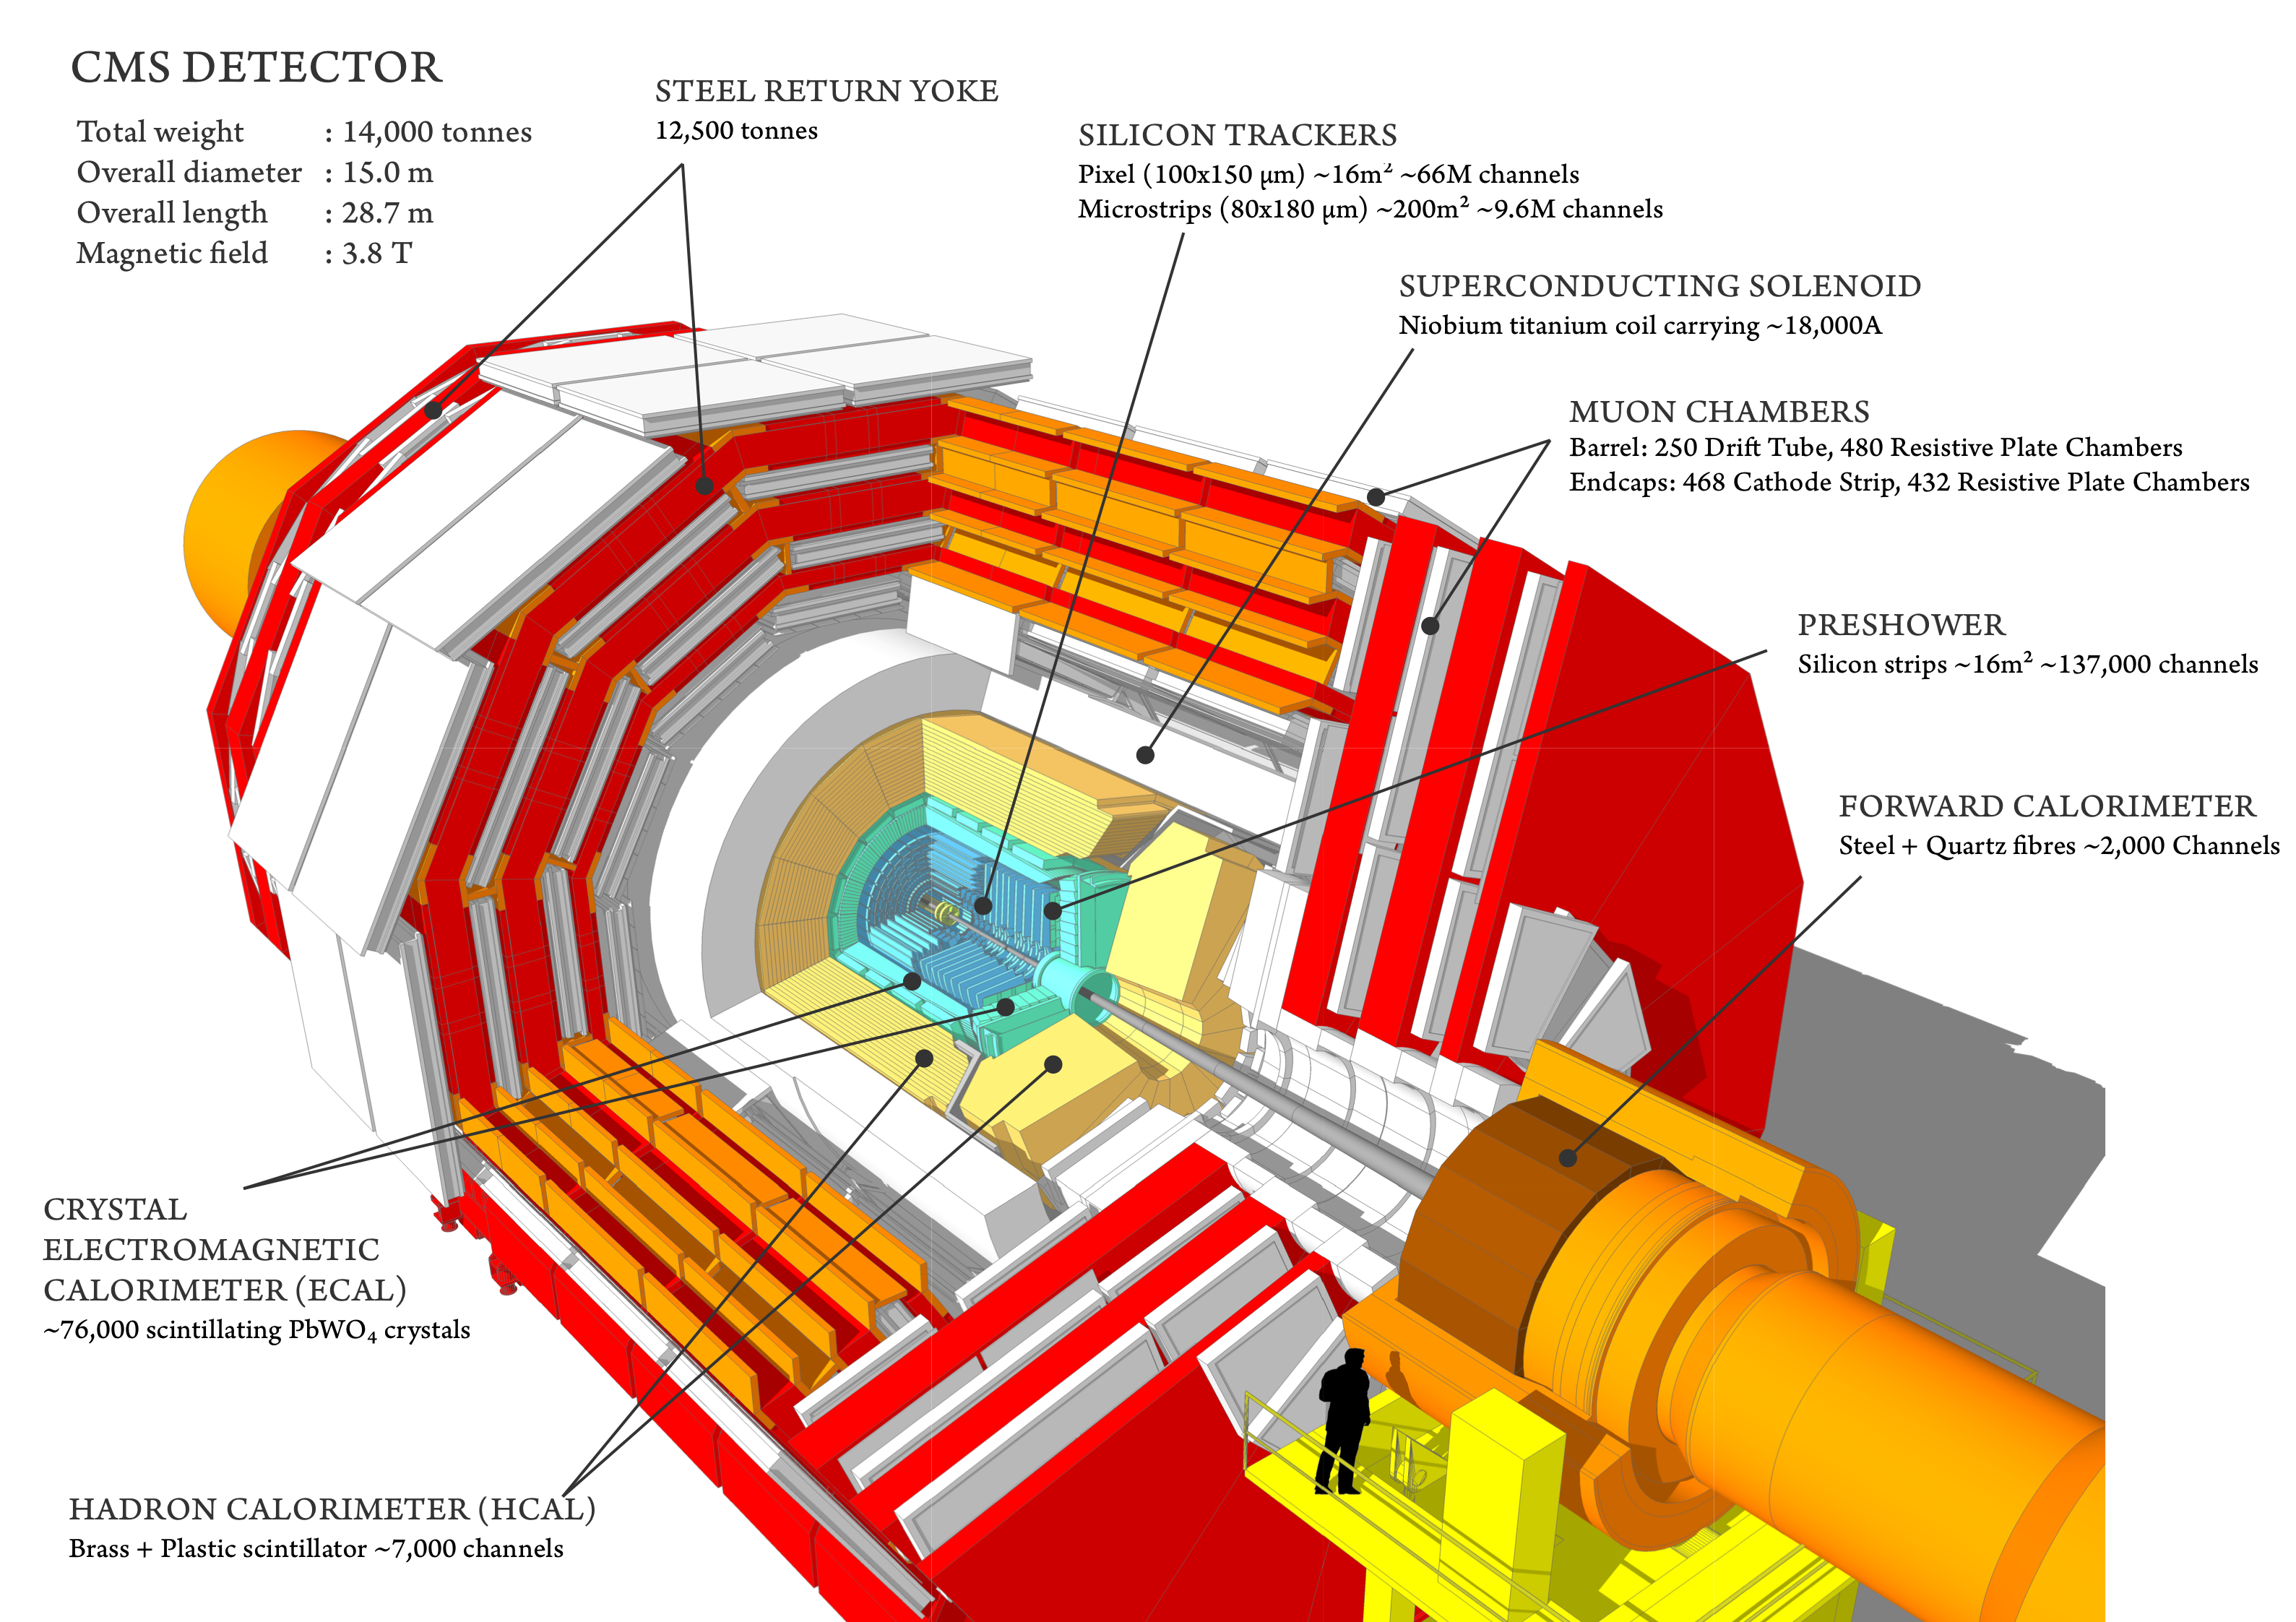
\includegraphics[width=0.95\textwidth]{figures/LHC/cms_120918_03.png}
	\caption{CMS detector drawing}
	\label{fig:CMS-detector}
\end{figure}

%%%%%%%%%%%%%%%%%%%%%%%%%%%%%%%%%%%%%%%%%%%%%%%%%%%%%%%%%%%%%%%%%%
%%%%%%%%%%%%%%%%%%%%%%%%%%%%%%%%%%%%%%%%%%%%%%%%%%%%%%%%%%%%%%%%%%
\subsection{CMS sub-systems} % (fold)
\label{sub:cms_sub_systems}

%%%%%%%%%%%%%%%%%%%%%%%%%%%%%%%%%%%%%%%%%%%%%%%%%%%%%%%%%%%%%%%%%%
%%%%%%%%%%%%%%%%%%%%%%%%%%%%%%%%%%%%%%%%%%%%%%%%%%%%%%%%%%%%%%%%%%
\subsubsection{Magnet} % (fold)
\label{ssub:magnet}
Magnet system of CMS consists of a superconducting solenoid magnet with 3.8 T magnetic field. It is 12.5 m in length and 6 meter in inner diameter. The high mangnetic field ensures the appropriate bending power of the high-energy charged particles to precisely measure its momentum. It is shown in Figure~\ref{fig:CMS-magnet}.

\begin{figure}[!htbp]
	\centering
	\includegraphics[width=0.95\textwidth]{figures/LHC/CMS_magnet.jpg}
	\caption{CMS Magnet system}
	\label{fig:CMS-magnet}
\end{figure}

% subsubsection magnet (end)
%%%%%%%%%%%%%%%%%%%%%%%%%%%%%%%%%%%%%%%%%%%%%%%%%%%%%%%%%%%%%%%%%%
%%%%%%%%%%%%%%%%%%%%%%%%%%%%%%%%%%%%%%%%%%%%%%%%%%%%%%%%%%%%%%%%%%
\subsubsection{Tracker} % (fold)
\label{ssub:tracker}
% subsection tracker (end)

%%%%%%%%%%%%%%%%%%%%%%%%%%%%%%%%%%%%%%%%%%%%%%%%%%%%%%%%%%%%%%%%%%
%%%%%%%%%%%%%%%%%%%%%%%%%%%%%%%%%%%%%%%%%%%%%%%%%%%%%%%%%%%%%%%%%%
\subsubsection{The Electromagnetic Calorimeter} % (fold)
\label{sub:the_electromagnetic_calorimeter}
% subsection the_electromagnetic_calorimeter (end)

%%%%%%%%%%%%%%%%%%%%%%%%%%%%%%%%%%%%%%%%%%%%%%%%%%%%%%%%%%%%%%%%%%
%%%%%%%%%%%%%%%%%%%%%%%%%%%%%%%%%%%%%%%%%%%%%%%%%%%%%%%%%%%%%%%%%%
\subsubsection{The Hadronic Calorimeter} % (fold)
\label{sub:the_hadronic_calorimeter}
% subsection the_hadronic_calorimeter (end)

%%%%%%%%%%%%%%%%%%%%%%%%%%%%%%%%%%%%%%%%%%%%%%%%%%%%%%%%%%%%%%%%%%
%%%%%%%%%%%%%%%%%%%%%%%%%%%%%%%%%%%%%%%%%%%%%%%%%%%%%%%%%%%%%%%%%%
\subsubsection{The Muon System} % (fold)
\label{sub:the_muon_system}

% subsection the_muon_system (end)
% subsection cms_sub_systems (end)



% \subsection{Detector Design} % (fold)
% \label{sub:detector_design}

% % subsection cms_detector_design (end)
% CMS\cite{paper:JINST:CMSCollaboration} detector is a general purpose deetector which consist of layers of material that exploit the different properties of particles to catch and measure the energy and momentum of each particles passing through it. So, CMS needs:
% \begin{itemize}
% 	\item a high quality central tracking system to give accurate momentum measurements with good efficienccy of offline tagging of b-jets and $\tau$'s.
% 	\item a high resolution ($\approx$ 1\% at 100 GeV) method to detect and measure electrons and photons (an electromagnetic calorimeter) and isolate them.
% 	\item a ``hermetic” hadron calorimeter, designed to entirely surround the collision and prevent particles from escaping along with fine lateral segmentation.
% 	\item a high performance system to detect and measure muons with good time and momentum resolution ($\approx$ 1\% at 100 GeV).
% \end{itemize}
% The CMS experiment has been built as a general purpose detector with excellent tracking and particle identification capabilities designed to fully explore the physics potential of the LHC. The CMS comprise the following sub-detectors:
% \begin{itemize}
% 	\item The inner tracking system is used for the identification and track measurement of charged particles.
% 	\item The electromagnetic calorimeter provides energy measurements. Electrons and photons deposit almost all of their energy in this sub-detector.
% 	\item Typically the interactions of hadronic jets imply that most of their energy is deposited after traversing more material than given by the electromagnetic calorimeter. The main energy component of these objects is measured with the hadronic calorimeter.
% 	\item The muon system identifies high energetic muons which can not be confined within the CMS experiment and measures their tracks and respective momenta.
% \end{itemize}





% % section cms_experiment (end)

% %%%%%%%%%%%%%%%%%%%%%%%%%%%%%%%%%%%%%%%%%%%%%%%%%%%%%%%%%%%%%%%%%%
% \section{CMS Trigger and Data Acquisition system} % (fold)
% \label{sec:cms_trigger_and_data_acquisition_system}

% % section cms_trigger_and_data_acquisition_system (end)

% %%%%%%%%%%%%%%%%%%%%%%%%%%%%%%%%%%%%%%%%%%%%%%%%%%%%%%%%%%%%%%%%%%
% \section{CMS Offline Computing} % (fold)
% \label{sec:cms_offline_computing}

% section cms_offline_computing (end)




% \begin{figure}[!htbp]
% 	\centering
% 	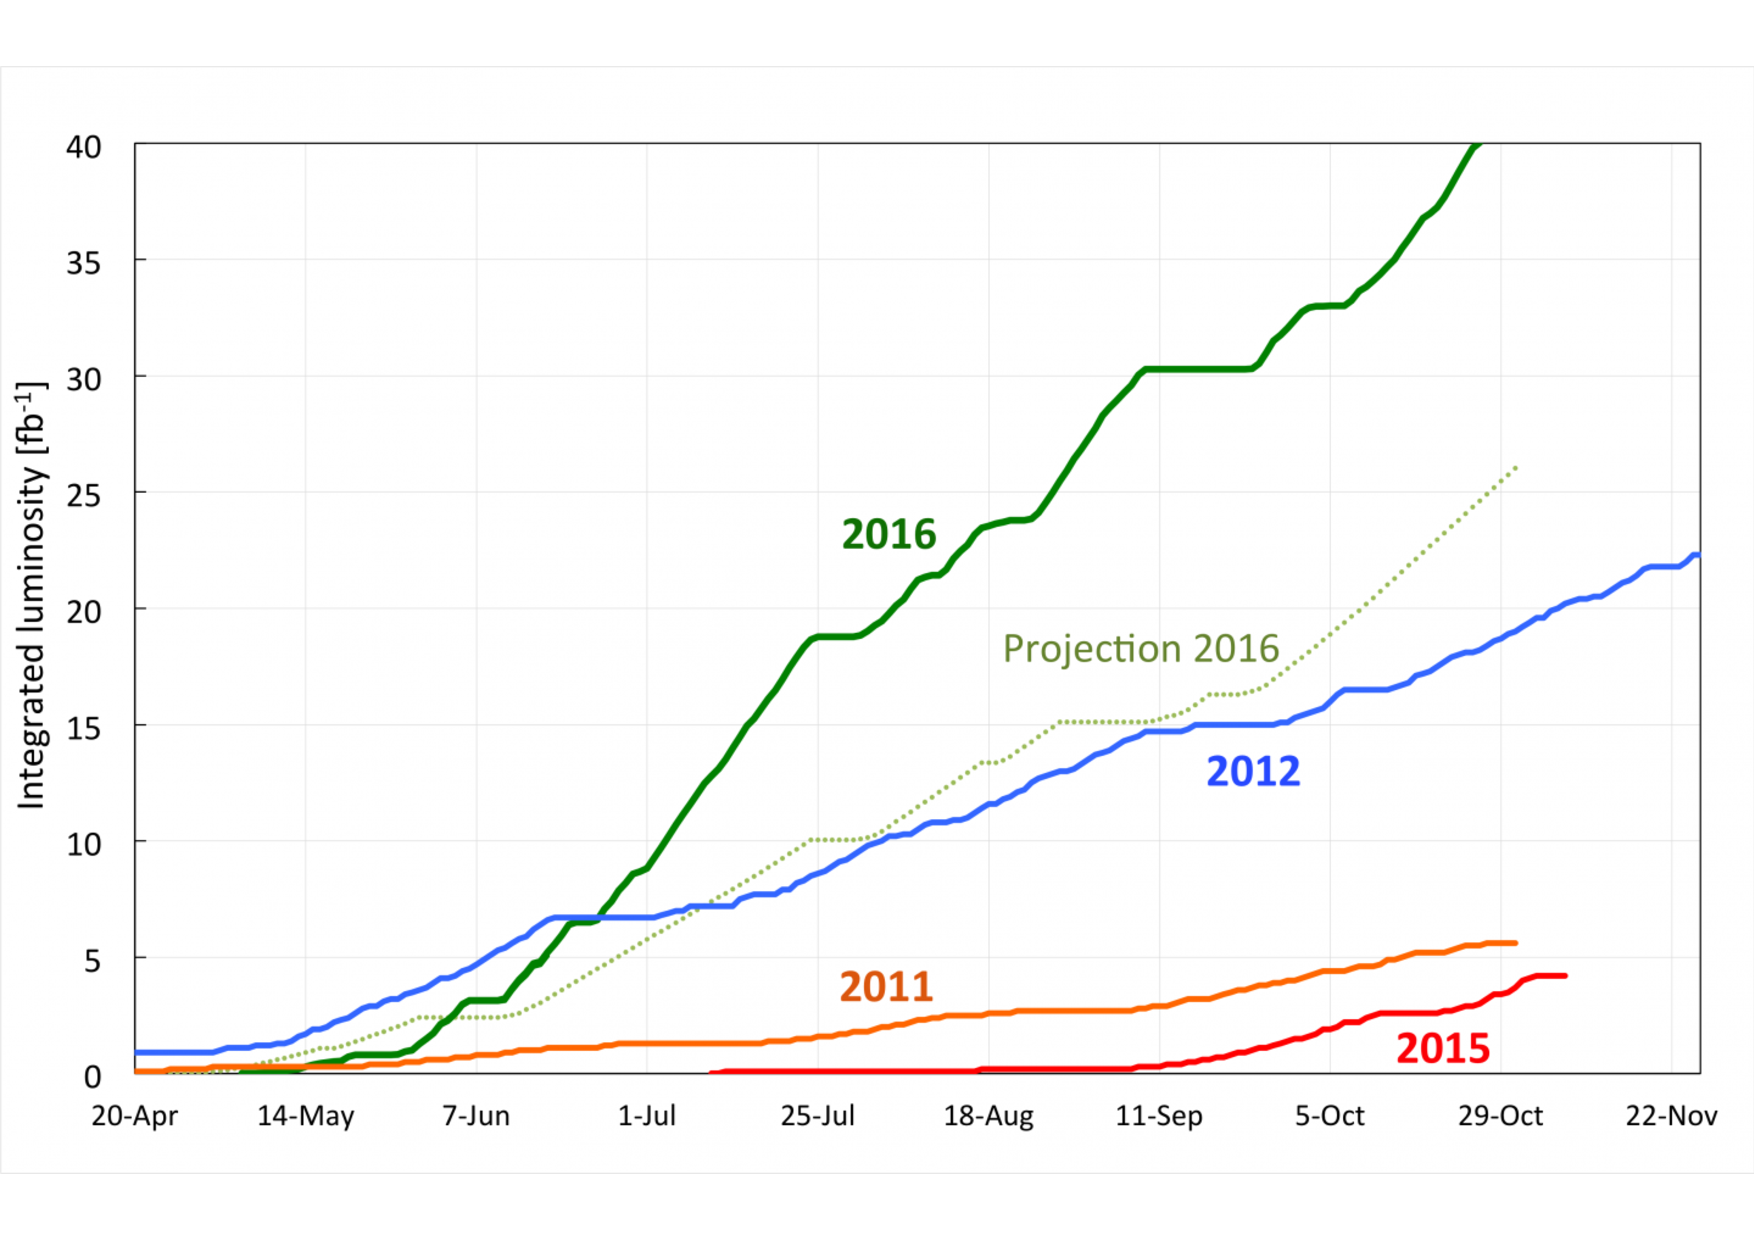
\includegraphics[width=0.95\textwidth]{figures/lumi-proj-2016-final-v2}
% 	\caption{The integrated luminosity of the LHC with proton-proton collisions in 2016 compared to previous years. Luminosity is a measure of a collider’s efficiency and is proportional to the number of collisions. The integrated luminosity achieved by the LHC in 2016 far surpassed expectations and is double that achieved at a lower energy in 2012. (Image : CERN)\todo[inline]{Update the caption.}}
% 	\label{fig:lumi-proj-2016-final-v2}
% \end{figure}



% \section{Other Information to be organized}



% The interaction in HEP experiments are characterized mainly by the center of mass energy along with type and number of particles.


% Because of limited geometrical space in LHC ring the beam pipe was designed as a ``twin-aperture" magnets, where superconducing ring is housed in a common return yoke and cryostat.

% chapter the_lhc_and_cms_machine (end)


% The CMS is a general-purpose detector at the LHC. It is built around a huge solenoid magnet. This takes the form of a cylindrical coil of superconducting cable that generates a field of 4 Tesla, about 100,000 times the magnetic field of the Earth. The field is confined by a steel ``yoke'' that forms the bulk of the detector's 12,500-tonne weight. The complete detector is 21 meters long, 15 meters wide and 15 meter high.


% \begin{figure}[!htbp]
% 	\centering
% 	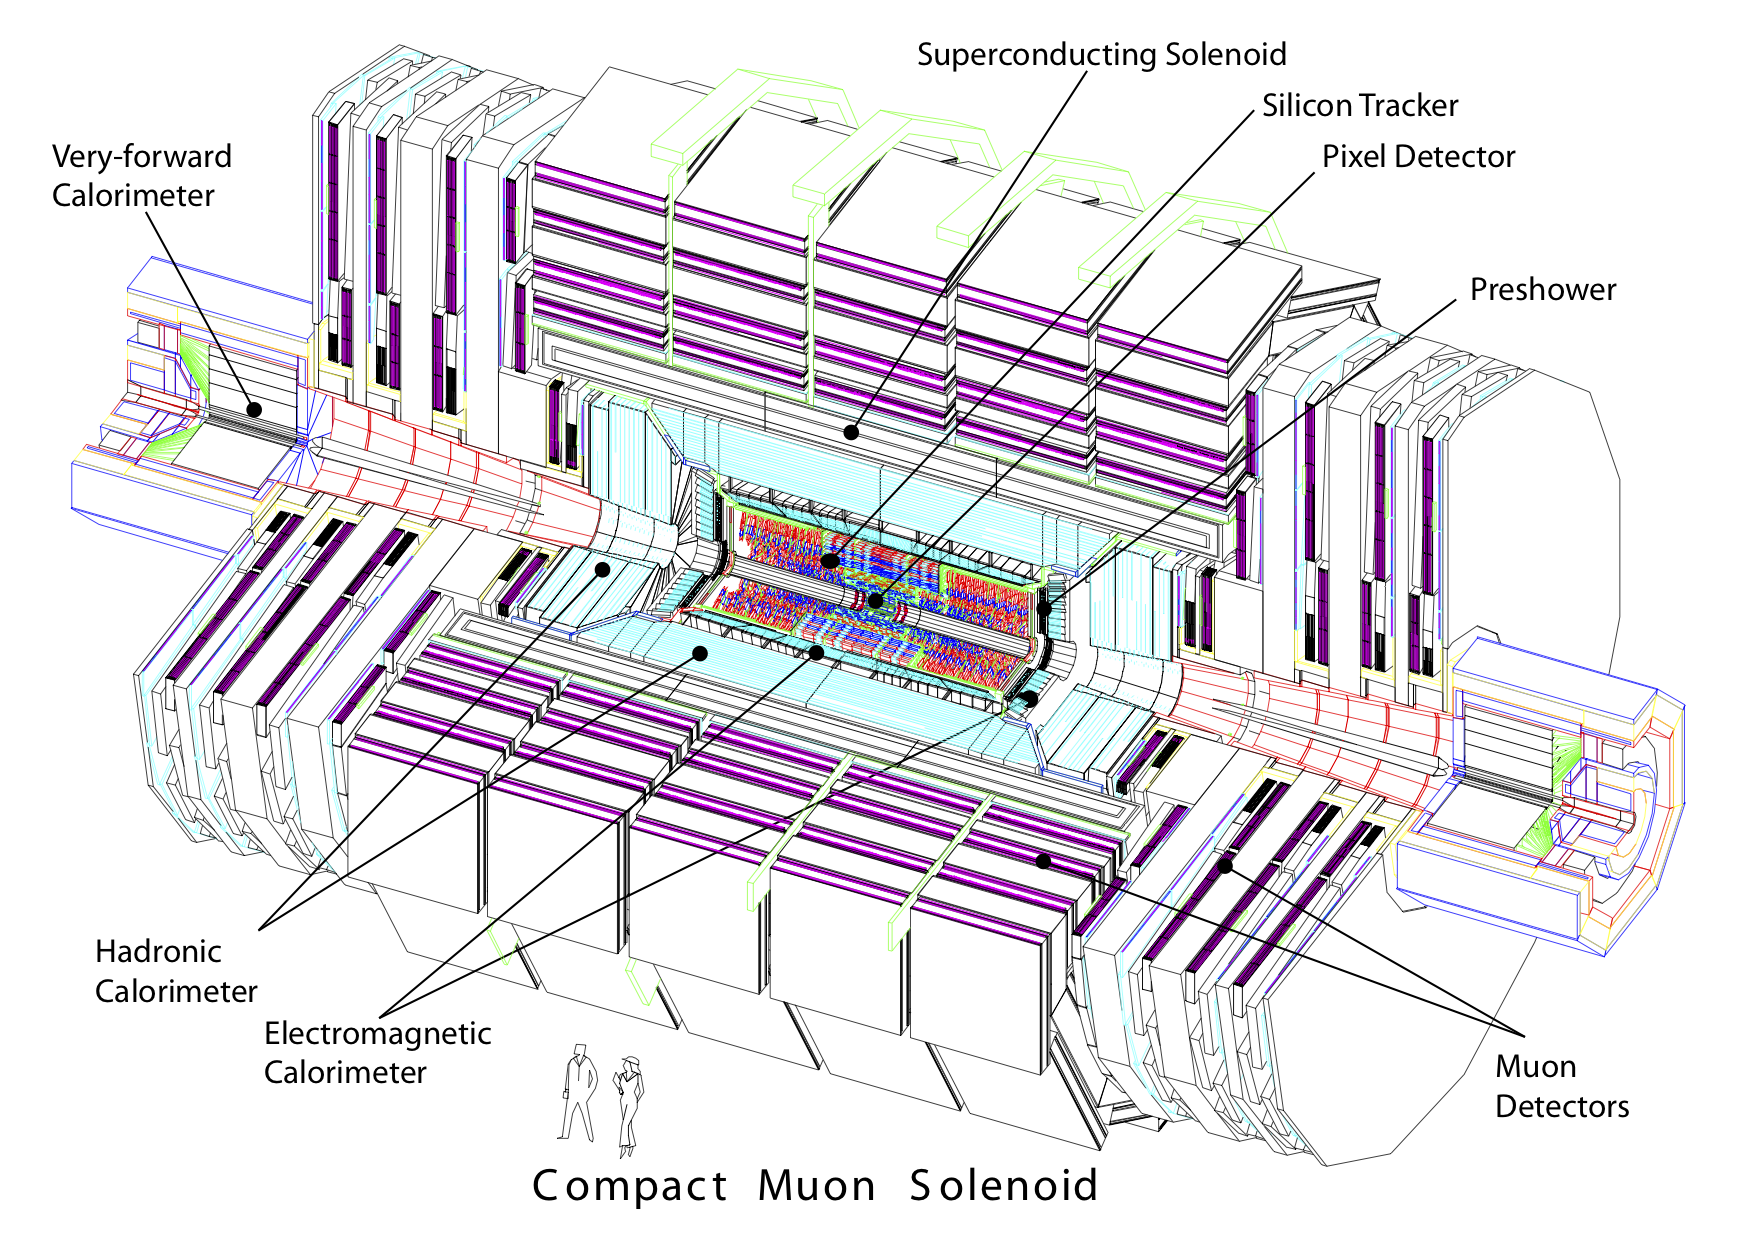
\includegraphics[width=0.95\textwidth]{figures/LHC/cms_complete_labelled.png}
% 	\caption{CMS detector drawing}
% 	\label{fig:CMS-detector-2}
% \end{figure}
